\documentclass[a4paper, 11pt]{report}

\usepackage[utf8]{inputenc}
\usepackage[francais]{babel}
\usepackage[T1]{fontenc}
\usepackage[final]{pdfpages}
\usepackage{graphicx}
\usepackage{parskip}
\usepackage{hyperref}
\usepackage{caption}
\usepackage{subcaption}
\usepackage{wrapfig}
\usepackage{epstopdf}
\usepackage{listings}
\usepackage{multicol}

\DeclareGraphicsRule{.eps}{pdf}{.pdf}{`epstopdf #1}
\pdfcompresslevel=9

\title{Éco-conception de logiciels\\ \large Rapport de stage de 5ème année}
\author{Guillaume Delamare}
\date{\today}

\begin{document}
\renewcommand{\labelitemi}{$\bullet$}
\renewcommand{\labelitemii}{$\diamond$}
\renewcommand{\labelitemiii}{$\ast$}
\renewcommand{\labelitemiv}{$\cdot$}

\maketitle

\tableofcontents

\chapter{Introduction}
%TODO Écrire le chapitre "Introduction"
% Présenter l'exercice du PRED
% Contexte de rattrappage

\chapter{Sujet}
	\section{Contexte}
Comme préciser dans le chapitre précédent, ce travail s'inscrit dans le cadre d'un rattrapage d'unité d'ensegnement de mon semestre 9. Je l'effectue durant le semestre 10 de ma formation. Ce semestre est dédié au stage de fin de formation. C'est donc durant mon stage que je le réalise. Le sujet traité dans ce travail est étroitement lié à celui que j'effectu en stage. Je dois donc commencer par le décrire avant de pouvoir expliquer le sujet ainsi que les objectifs du travail dont ce rapport fait l'objet.

Mon stage se déroule dans le l'équipe ASCOLA au sein de l'école des Mines de Nantes. Cette équipe fait partie du LINA\footnote{Laboratoire d'informatique de Nantes Atlantique} ainsi que de l'INRIA\footnote{Institut National de Recherche en Informatique et Automatique}. Je suis encadré par Thomas Ledoux, enseignant chercheur à l'école des mines.

Pour résumer, mon stage consiste à définir des axes de recherches et à explorer des pistes afin de mettre en valeur les possibilités offertes par une approche écologique de la conception de logiciel. Pour être plus précis, je travail sur différents aspect de la fabrication de logiciel et de la maitrise de la consommation d'énergie par les systèmes d'informations. Pour la première partie, cela va de la conception à l'execution. Pour la deuxième partie, je travail principalement sur la mesure de consommation d'un logiciel et un peu sur les aspect d'analyse du cycle de vie.


	\section{Sujet}
Avec la montée en puissance de l’informatique dans les nuages, il est nécessaire de renforcer l’infrastructure sur laquelle repose cette technologie. La première conséquence est le besoin, grandissant, en nouveaux centres de données. Afin de limiter cette multiplication, différentes actions ont été entreprises afin de rationaliser l’utilisation de ceux existant (virtualisation, migration de données à chaud...). Cependant, cela n'empêche pas les centres de données de consommer toujours plus d’énergie et d’atteindre en 2010 entre 1,1\% et 1,5\% de la consommation mondiale d’électricité \footnote{voir : http://www.analyticspress.com/datacenters.html}.

Afin de pouvoir réduire les besoins en énergie de ces centres de données, il est important de mieux comprendre comment ils consomment. Pour cela une étude plus détaillée des composants mis en action dans l’utilisation des serveurs, apparaît comme évidente.

Ce projet propose d’étudier plus particulièrement la consommation des disques durs sous différentes configurations (technologie RAID, système de fichiers...). Afin de compléter l’étude de l’impact énergétique, il faudra y concaténer d’autres études sur la fabrication et la mise en déchet de ces mêmes disques durs. Cela nous permettra d’avoir un point de vue global de type ACV (Analyse du Cycle de Vie) sur ce composant particulier.
	
	\section{Objectif}
		\subsection{Recherche bibliographique}
\begin{itemize}
	\item Recherche d’études préalables.
	\item Recherche d’informations sur la consommation du produit aux étapes de fabrication et de mise en déchet.
\end{itemize}

		\subsection{Réalisation}
\begin{itemize}
	\item Définir une méthodologie de mesure de la consommation d’un disque dur.
	\item Développer une collection de tests permettant d’effectuer des mesures sur les disques durs.
	\item Réaliser ces tests sur plusieurs architectures de disques.
\end{itemize}

\chapter{État de l'art}
	\section{Introduction}

	\section{La mesure de consommation d'énergie}
Dans cette partie de l'état de l'art je vais parler des différentes techniques pour extraire et utiliser une information sur la consommation d'un logiciel. J'ai pu identifier trois méthodes différentes pour mesurer l'énergie consommée. Elles ont chacunes leurs avantages et leurs défauts.
			\subsection{La mesure par un appareil externe}
La première méthode, la plus commune pour mesurer les resources consommées par un appareil électrique, est de placer un wattmètre en série sur l'alimentation de cet appareil. Avec un wattmètre récent on peut mesurer un ensemble de paramètre tels que les watts, les watts/heure, les volts et les ampères. De plus, la plupart des outils récents proposent un système d'enregistrement et/ou de transfert des données vers un ordinateur.

\begin{wrapfigure}{dR}{0.3\textwidth}
		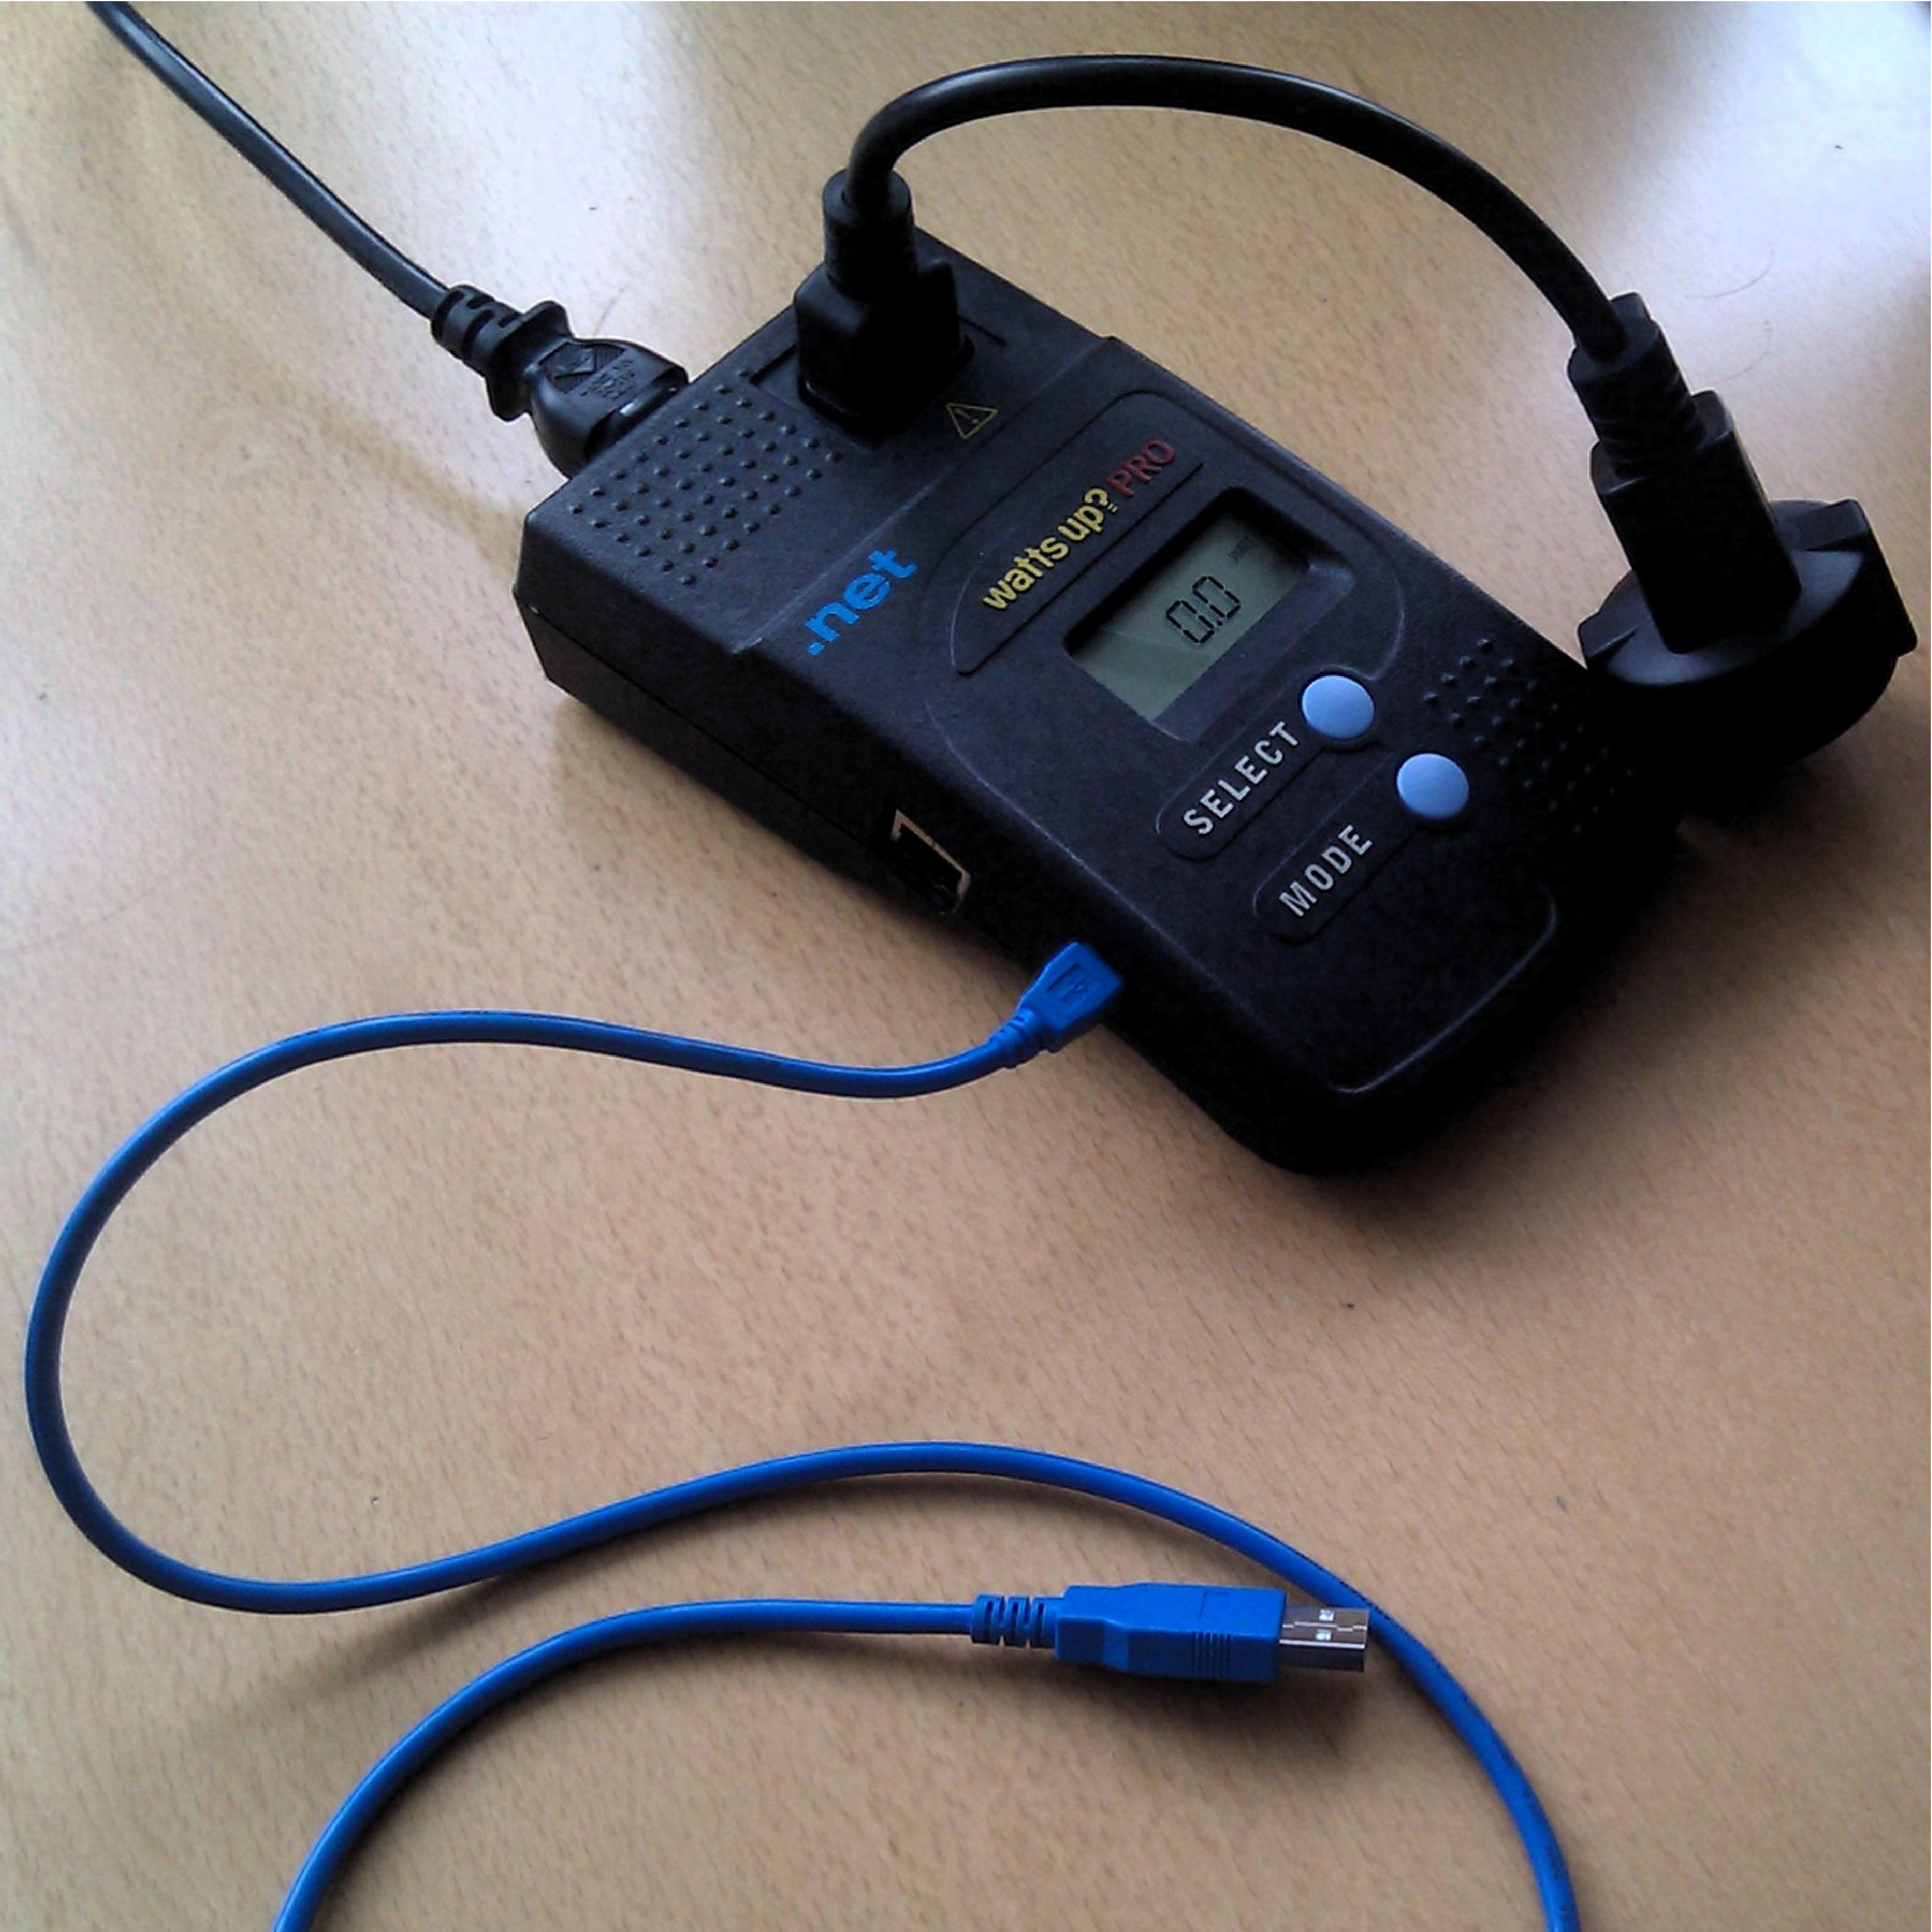
\includegraphics[width=0.3\textwidth]{figures/wattsUp}
		\caption{Photo d'un watts up pro .net}
		\label{wattsUp}
\end{wrapfigure}

Par exemple, les \textit{plugwizes} sont des modules qui se placent sur la prise sont capables de couper l'alimentation de l'appareil branché dessus et de mesurer la consommation électrique de celui ci. Ils sont capable de transmettre ces informations sans fil jusqu'à un ordinateur. Un autre exemple de ce type de matériel, les wattmètres de la marque \textit{watts up\/?}. Ils permettent, suivant leur gamme, de collecter de l'information et de la transmettre. Le \textit{watts up\/? pro .net} (figure~\ref{wattsUp}) dispose d'un système d'enregitrement de, au maximum, 120000 mesures de watts et de deux interface de communication, USB et Ethernet.

Cette technique de mesure n'offre qu'une vue globale de notre système. Il est impossible par cette méthode d'identifier de manière certaine la consommation d'un logiciel. On peut par contre corréler un changement de consommation avec un événement survenu\cite{GreenMining} (le démarrage d'une application, le lancement d'une tâche gourmande en traitement\ldots). 

			\subsection{La mesure par un logiciel interne}
La deuxième méthode consiste à analyser les ressources utilisées par un programme et, à partir d'un modèle de consommation, d'en déduire la consommation énergétique de l'application\cite{da2010methodology}. Différentes ressources peuvent être ciblées. On peut les classer en deux catégories ~: les unités de calcul (CPU, GPU\ldots) et les dispositifs d'entrées/sorties (disque dur, interface réseau\ldots).

Dans cet article\cite{noureddine:hal-00681560}, les auteurs détaillent le modèle de consommation qu'ils ont mis au point pour leur application de mesure \textit{PowerAPI}. On peut y voir qu'ils obtiennent des résultats intéressants par rapport à la mesure faite en parallèle sur un wattmètre. L'inconvénient de ce type de méthode est qu'il faut calibrer le modèle. Cela est nécessaire car chaque processeur  fonctionne différemment et donc ne consomme pas la même chose. De plus ce type de méthodes est intrusive et peut perturber le fonctionnement du logiciel.

En revanche cette technique permet facilement d'isoler un logiciel en particulier (ou plutôt un processus). C'est donc une technique intéressante pour mon projet.

			\subsection{Vers une mesure par un appareil interne}
Enfin une troisième technique est à envisager dans un futur plus ou moins proche. Comme l'explique l'article \textit{Looking back on the language and hardware revolutions
~: measured power, performance, and scaling}\cite{Esmaeilzadeh:2011:LBL:1950365.1950402}, les fabricants de matériel intègrent, de plus en plus, dans leurs composants, des mécanismes de mesure afin d'adapter leurs fonctionnements à leurs consommations. À la fin de l'article, les auteurs recommandent l'ouverture de ces mécanismes au travers d'API pour que les développeurs puissent y accéder.

Si les constructeurs acceptent de faire cet effort, on pourra facilement savoir ce que consomme réellement une application en temps réel. Ce type de mécanisme serait idéal dans mon projet car il permettrait d'avoir une consommation réelle de l'application mesurée. On pourrait même concevoir, très facilement, des applications qui s'adaptent en fonction de leur consommation.

	\section{Logiciels de mesure}
Dans cette section je vais présenter les logiciels de mesure de consommation que j'ai pu essayer. Je présenterais leurs avantages et leurs défauts.
		\subsection{ClassMexer}
ClassMexer\footnote{\href{http://www.javamex.com/classmexer/}{www.javamex.com/classmexer/}} est un API java permettant d’estimer la taille en mémoire d’un objet java. On peut télécharger cet API sous la forme d’un fichier JAR sur son site internet. ClassMexer est un \textit{Instrumentation agent} comme spécifié dans le pattern Instrument\footnote{\href{http://docs.oracle.com/javase/6/docs/api/java/lang/instrument/package-summary.html}{docs.oracle.com/javase/6/docs/api/java/lang/instrument/package-summary.html}}. Cela implique de travailler avec, au minimum, la version 5 de java.

			\subsubsection{procédure d'installation}
\begin{itemize}
	\item Télécharger l’API
	\item Importer le fichier JAR dans le projet.
	\item Insérer des appels sur l’objet que l’on souhaite mesurer. Par exemple ~:
\begin{lstlisting}[language=Java]
public class Main {
   public static void main(String[] args) {
      String str="Hello world !";

      long noBytes=MemoryUtil.deepMemoryUsageOf(str);

      System.out.println(noBytes);
   }
}
\end{lstlisting}
	\item Exécuter le programme avec l’option -javaagent:<fichier JAR>
\end{itemize}

		\subsection{JouleMeter}
\textit{JouleMeter}\footnote{\href{http://research.microsoft.com/en-us/downloads/fe9e10c5-5c5b-450c-a674-daf55565f794/}{research.microsoft.com/en-us/downloads/fe9e10c5-5c5b-450c-a674-daf55565f794/}} est un outil développé par Microsoft et qui sert à mesurer la consommation d’énergie sur un ordinateur. Il ne fonctionne que sous Windows 7.

			\subsubsection{Procédure d'installation}
\begin{itemize}
	\item Télécharger le logiciel sur son site.
	\item Exécuter le programme.
\end{itemize}

			\subsubsection{Fonctionnement}
\textit{JouleMeter} est un logiciel de mesure qui se base sur un modèle de consommation. La première étape est donc de générer ce modèle. Deux méthodes existent.

La première n’est utilisable que sur un ordinateur portable muni d’une batterie. Il suffit de débrancher l’alimentation et de lancer la calibration (15 minuntes sans utiliser le PC). Avant de lancer la calibration, il faut faire attention à arrêter toutes les applications afin que le logiciel puisse déterminer une consommation minimum en mode "Idle".

Le deuxième mode nécessite un Wattmètre WattsUp pour générer le modèle. Il suffit de le brancher en USB, de couper toutes les applications possibles et de lancer la calibration (3 minutes sans utiliser le PC).

			\subsubsection{Expérience}
Afin de tester la fiabilité du modele créé, j'ai effectué différentes expériences en comparant les résultats obtenu par \textit{JouleMeter} avec ceux lu sur un wattmètre. J'ai pu mettre en évidence de grosses faiblesses qui rendent peu fiable les résultats obtenu. La figure~\ref{joulemeter} met en évidence ces faiblesses. J'ai obtenu ces mesures en laissant fonctionner \textit{JouleMeter} sur un ordinateur, démaré mais inutilisé, durant toute une nuit. En parallèle, j'ai récupéré les mesures que prenait un wattmètre \textit{WattsUp pro}.

\begin{figure}
	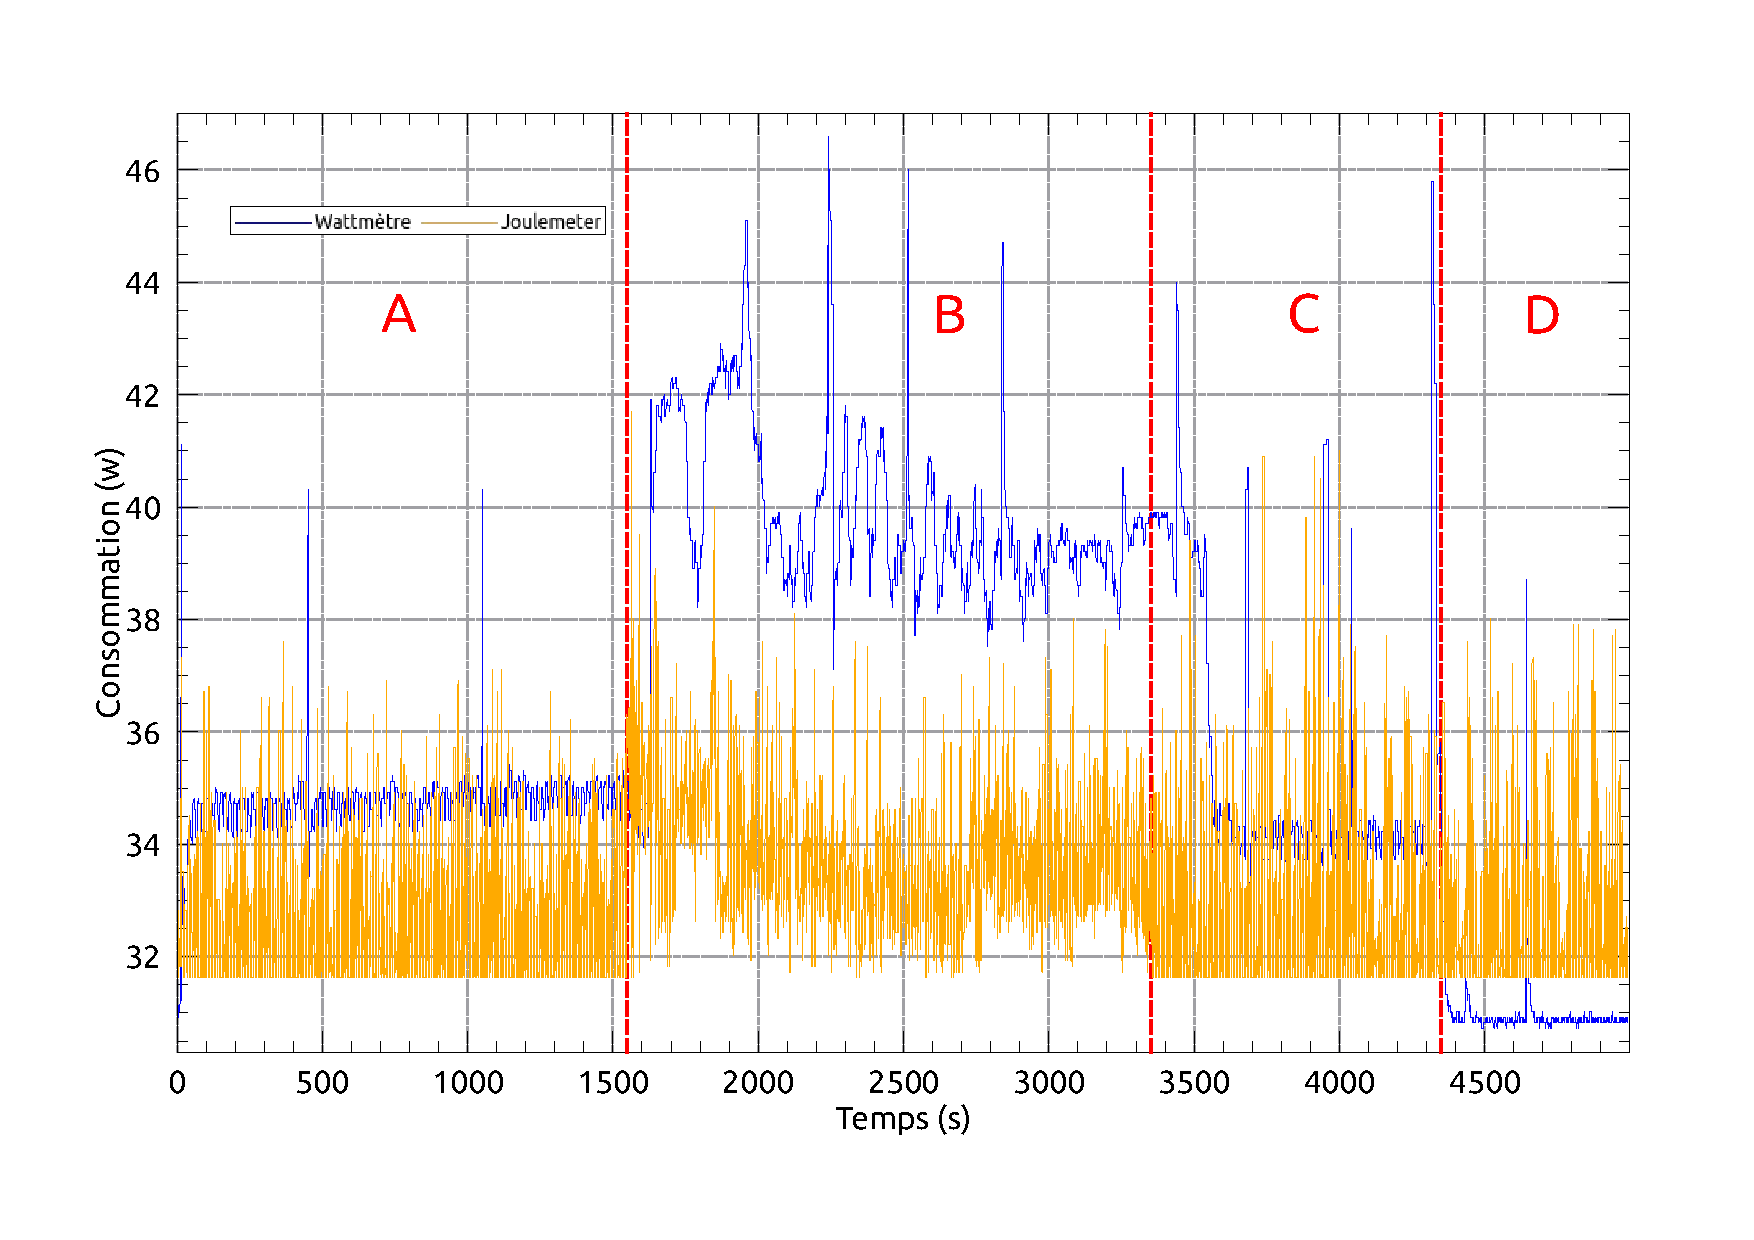
\includegraphics[width=0.99\textwidth]{figures/joulemeter.pdf}
	\caption{Mesures faites par Joulemeter comparé à celles d'un wattmètre}
	\label{joulemeter}
\end{figure}

Les deux coubes affichent un échantillon  de 5000 mesures (durant approximativement 5000 secondes). Le modèle de consommation sur lequel se basait \textit{JouleMeter} a été généré juste avant le début de l'expérience. D'un point de vue général, on peut déjà remarquer que la courbe de \textit{JouleMeter} est très irrégulière et majoritairement en dessous de celle du watttmètre. Cela est principalement du, au fait que l'impact du processeur est largement sous-estimé dans le modèle.

Ensuite on peut noter un seuil en dessous du quel \textit{JouleMeter} ne descend pas (ici, 31,6 watts). On constate même que les mesures du wattmètre passe en dessous de celle de \textit{JouleMeter} dans la partie \textit{D} du graphique. Cet effet de seuil est engendré par le modèle qui considère que le système consomme toujours une constante quand il est allumé. Donc, quelle que soit la charge du système, \textit{JouleMeter} considère qu'il consomme au minimum 31,6 watts (valeur qu'il a mesuré lors de l'établissement du modèle).

Enfin, et tout n'est pas négatif, on peut remarquer que dans la zone B \textit{JouleMeter} réussi à mesurer une hausse de la consommation qui peut être noté sur la courbe du wattmètre (avec un certain décalage cependant).

		\subsection{PowerAPI}
\textit{PowerAPI} est un outil sur lequel travail l'équipe ADAM de l'université de Lille. Les premiers résultats de cet outil ont été présentés dans un papier\cite{noureddine:hal-00681560} publié à l'ICSE\footnote{International Conference on Software Engineering} 2012 à Zurich. Cet outil parait prometteur et s'il continue à être développé, pourrait bien apporter une solution intéressante au problème de la mesure de consommation énergétique de logiciel.

Selon la présentation qui en a été faite, il fonctionne actuellement pour la consommation CPU. Cet outil collecte le temps CPU d'un processus et la fréquence de celui-ci en temps réel. Puis il détermine l'énergie consommée grâce à des tables de consommations par rapport à la fréquence fournis par les fabriquant de processeur.

Je n'ai malheureusement pas essayé \textit{PowerAPI} par manque de temps. Je n'ai eu accès au programme que tardivement durant mon stage et à ce moment je travaillais sur d'autres aspects.
	
	\section{Un composant central des systèmes d'information : le disque dur}
	%TODO Écrire la section "Un composant central des systèmes d'information : le disque dur"
Dans ce travail, je vais me concentrer sur un composant particulier : le disque dur. C'est pourquoi, dans cette troisième partie, je vais présenter certaines notions sur le fonctionnement d'un disque dur. Je vais développer trois sujet. 

Tout d'abord, je vais parler des systèmes de fichier qui sont le moyen utilisé par le système d'exploitation pour organiser l'information sur un disque. Ensuite, je parlerais de la technologie RAID qui définit des architectures de disque dur dans le but d'améliorer la rapidité d'accés au donnée ou la tolérance au panne d'un système de stockage. Enfin, je parlerais de la consommation d'un disque dur.
		
		\subsection{systèmes de fichiers}
			\subsubsection{FAT32}
			
			\subsubsection{NTFS}
			
			\subsubsection{EXT2}
			
			\subsubsection{EXT3}
			
		\subsection{La technologie Raid}
RAID est une technologie permettant de répartir les données stockées sur plusieurs disque dur. Le but peut être d'augmenter la tolérance aux pannes par l'introduction de redondance, d'améliorer la rapidité d'accés au données ou encore de sécuriser les données. Le terme RAID a été définit dans l'article \textit{A Case for Redundant Arrays of Inexpensive Disks (RAID)}\cite{Patterson:1988:CRA:50202.50214}. Dans cette article est proposé la définition de 5 niveaux de RAID
			\subsubsection{RAID 0}
			
			\subsubsection{RAID 1}
			
			\subsubsection{RAID 5}
		
		\subsection{Consommation d'un disque dure}
		
	\section{Conclusion}

\chapter{Propositions de réalisations}
	\section{Réalisation de mesure sur différentes architectures de disque dur}
		\subsection{Description}
L'idée de cette contribution serait de réaliser différentes installation de disque dur en variant l'architecture (RAID), le système de fichier (NTFS, ext2, ext3\ldots) et de procéder à une étude de leurs consommations. Il faudra donc mettre en place un banc d'éssais, c'est à dire un jeu d'instruction à exécuter sur chaques installation ainsi qu'un système de mesure qui permettra de récupérer les information de consommation.

		\subsection{Technologie à mettre en place}
Pour cette réalisation, j'aurais besoin de matériels, à commencer par suffisament de disques dur pour réaliser les installations que l'on souhaite tester. Il faudra aussi le matériel nécéssaire pour mesurer la consommation de nos installations. Un wattmètre devrait suffire à partir du moment on il nous permet d'isoler la consomation des disque dur. Il faut donc pouvoir le brancher directement sur l'alimentation du disque.  

	\section{Création d'un logiciel d'estimation de la consommation d'un disque dur}
		\subsection{Description}
Durant mon stage, j'ai été surpris de constater que les logiciels de mesure de la consommation ne prenaient pas en compte les accés au disque. Pour cette contribution, l'idée est de partir des résultats obtenus par Anthony Hylick, Ripduman Sohan, Andrew Rice, and Brian Jones\cite{hylick2008analysis} pour établir un model de consomation. Ensuite je pourais créer un logiciel estimant en temps réel la consommation d'un disque dur sur le même principe que powerAPI\cite{noureddine:hal-00681560}.

		\subsection{Technologie à mettre en place}
Pour la réalisation de cette application il faut utiliser une bibliothèque permettant la capture des lectures/écritures sur un disque au niveau du système d'exploitation. Une première recherche m'a mis sur la piste de SYSSTAT\footnote{\href{http://sebastien.godard.pagesperso-orange.fr/}{http://sebastien.godard.pagesperso-orange.fr/}}. C'est un ensemble d'outils pour les systèmes Linux qui permet surveiller un certain nombre de paramètres du système, entre autres, les entrées/sorties sur les disques.

Afin de valider complétement le modèle développé au sein de ce logiciel, il faudra aussi mettre en place un système de mesure de la consommation réel. Comme pour la contribution précédente, un wattmètre qui peut se brancher sur les disques sera suffisant.

\chapter{Réalisation}
A venir.

\chapter{Conclusion}
%TODO Écrire le chapitre "Conclusion"

\bibliographystyle{plain}
\bibliography{biblio}
\listoffigures{}
\listoftables{}

\appendix

\end{document}